%==============================================================================
%  Paper 1, the fire spread model (fitting + validation)
%  Target: International Journal of Wildland Fire (CSIRO Publishing)
%  Type:   RESEARCH ARTICLE
%
%  ---------------------------------------------------------------------------
%  COMPLIANCE SUMMARY, full rules + sources in guidelines/IWJF_guidelines.md
%  ---------------------------------------------------------------------------
%   [ ] MAIN TEXT   <= 6000 words, Introduction -> Conclusion ONLY.
%                   Excluded: title, abstract, references, figure captions, tables.
%                   Check with:  make words
%   [ ] ABSTRACT    <= 200 words, STRUCTURED, exactly these labels, in order:
%                   Background; Aims; Methods; Key results; Conclusions; Implications.
%                   No citations, equations, lists, tables or figures.
%   [ ] KEYWORDS    >= 8 (checklist says "eight or more"). Also work them into
%                   the title and the abstract.
%   [ ] ONLINE SUMMARY  50-80 words, 3 sentences, jargon-free (optional for IJWF,
%                   but cheap and it is what shows up on the article landing page).
%   [ ] LINE NUMBERS  required, continuous -> class option `linenum' (below).
%   [ ] STATEMENTS  Data availability + Conflicts of interest + Declaration of
%                   funding are COMPULSORY. AI declaration if AI was used.
%   [ ] SPECIES     scientific name + authority at first mention, then be consistent.
%   [ ] UNITS       SI; one convention for rates (m s$^{-1}$ or m/s) throughout.
%   [ ] STATS       report package citations AND version numbers; state assumptions.
%   [ ] REFERENCES  Harvard (CSIRO). Full journal names, DOIs, >=3 authors then
%                   et al., no ellipses. Style file: samplebib.bst.
%   [ ] SUBMISSION  ScholarOne, cover letter, >= 3 suggested reviewers (no recent
%                   collaborators / same institution), preprint link if any.
%
%  NOTE: IJWF accepts FORMAT-FREE submission, the production team applies journal
%  style after acceptance. We use the CSIRO class anyway so the layout, the word
%  budget and the reference style are honest from the start.
%==============================================================================

\documentclass[ResearchPaper,linenum]{CSIRO_LaTeX_Template}

% --- Harvard punctuation: (Smith 2024; Doe 2025), no comma before the year ----
\bibpunct{(}{)}{;}{a}{}{;}

% The class does not load booktabs; the tables here use \toprule/\midrule/\bottomrule.
\usepackage{booktabs}

% --- Class fix: \subsubsection can collide with the preceding paragraph --------
% CSIRO_LaTeX_Template.cls line 1035 gives \subsubsection a beforeskip of
% "12pt \@plus -1pt": 12pt of space with NEGATIVE stretch. In a column the class
% stretches to fill the page, that glue shrinks instead of growing, and the
% heading rides up onto the last line of the paragraph above it (it did so to
% "Hierarchical structure"). Same definition, well-formed glue -- \subsection
% (line 1034 of the class) already uses this form.
\makeatletter
\renewcommand\subsubsection{\@startsection{subsubsection}{3}{\z@}%
  {12pt \@plus 1pt \@minus 1pt}{.1pt}{\subsubsectionfont}}
\makeatother

% --- Class fix: the ORCID icon beside an author name links nowhere -------------
% CSIRO_LaTeX_Template.cls line 726 defines \orc with the host and path swapped,
% "https://orcid/org/#1", so every icon in the byline points at a domain that does
% not exist. \auorc (line 773), used in the affiliations, has the URL right. Same
% definition, correct address.
\makeatletter
\def\orc#1{\href{https://orcid.org/#1}{\kern1pt\raisebox{-1.3pt}{%
  
\includegraphics[height=7pt]{Logos/orcid_logo_Web}}}}
\makeatother

\graphicspath{{figures/}{../figures/}}

\begin{document}

\journaltype{Research Article}
\jwebadd{https://doi.org/10.1071/WFxxxxx}
\journalname{International Journal of Wildland Fire}

%TC:ignore
%------------------------------------------------------------------------------
% TITLE, accurate, informative, brief; no abbreviations or formulae;
%         include keywords in it where possible.        [not counted in the 6000]
% NOTE: the %TC:ignore above opens here, not at the abstract, because the title, the
% author names and the affiliations are outside the 6000-word budget too. With it at
% the abstract, `make words' was counting them (~60 words once the real affiliations
% went in).
%------------------------------------------------------------------------------
\title{Fitting a hierarchical fire spread model based on fire polygons}

\versorh{Barberá}                                  % verso running head (author)
\rectorh{International Journal of Wildland Fire}   % recto running head

%------------------------------------------------------------------------------
% AUTHORS, full first and last names. Corresponding author gets *.
% ORCID: required for the submitting author, recommended for all. Co-authors MUST
% link their ORCID to their ScholarOne account BEFORE acceptance (cannot be added later).
%------------------------------------------------------------------------------

% Affiliation letters follow the AUTHOR ORDER, not the author count: Kitzberger shares
% affiliation A with Barbera, so there are five authors and four affiliations.
% Institution names are kept in their own language (they are proper nouns), with city,
% province and country in English -- the same form as Barbera et al. (2025) in Fire Ecology.
\author[A,*\orc{0000-0002-7572-4471}]{Iv\'an Barber\'a}
\author[B\orc{0009-0006-6216-3763}]{Iv\'an Renison}
\author[C]{Marcelo Bari}
\author[A\orc{0000-0002-9754-4121}]{Thomas Kitzberger}
\author[D\orc{0000-0001-7269-7490}]{Juan Manuel Morales}

\affil[A]{Instituto de Investigaciones en Biodiversidad y Medioambiente, CONICET and Universidad Nacional del Comahue, San Carlos de Bariloche, Río Negro, Argentina}{\auorc{0000-0002-7572-4471}{} \auorc{0000-0002-9754-4121}{}}
\affil[B]{Facultad de Matemática, Astronomía, Física y Computación, Universidad Nacional de Córdoba, Córdoba, Argentina}{\auorc{0009-0006-6216-3763}{}}
\affil[C]{Departamento de Incendios, Comunicaciones y Emergencias, Parque Nacional Nahuel Huapi, Administración de Parques Nacionales, San Carlos de Bariloche, Río Negro, Argentina}{}
\affil[D]{School of Biodiversity, One Health and Veterinary Medicine, University of Glasgow, Glasgow, United Kingdom}{\auorc{0000-0001-7269-7490}{}}


\corau{*Correspondence to: Email: ivanbarbera93@gmail.com}

%------------------------------------------------------------------------------
% ABSTRACT, 200 WORDS. Structured, these six labels, this order.
% No citations, no equations, no lists. Include the keywords. Define any
% abbreviation here AND again at first use in the body.
%------------------------------------------------------------------------------
\begin{abstract}
\textbf{Background.} Assessing fire regime trajectories under climatic and 
management scenarios needs fire spread models that 
can be fitted and validated where fire behaviour is poorly documented.
\textbf{Aims.} To develop and evaluate a fire spread model for north-western
Patagonia using regionally available inputs, and a fitting method
that needs only fire perimeters and ignition location.
\textbf{Methods.} We developed a stochastic cellular automaton where parameters
vary among fires in a hierarchical formulation. It was fitted with a novel strategy of
hierarchical Approximate Bayesian Computation, based on 57 fires with known
ignition location, with 178 further fires informing fire size.
\textbf{Key results.} Wind and slope dominated spread probability, with 
vegetation and topography showing smaller effects. Fire weather strongly 
controlled fire size.
Simulated fires reproduced the response of size to fire weather but were
larger and rounder than observed ones, a limitation of the contagion geometry.
\textbf{Conclusions.} The hierarchical, likelihood-free fitting approach recovers
realistic fire behaviour from perimeters alone, but the spread geometry should 
be replaced.
\textbf{Implications.} Combined with an elliptical spread geometry, the approach
offers a cheap, data-frugal way to build fire spread models to simulate fire regimes.
\end{abstract}

%------------------------------------------------------------------------------
% KEYWORDS, EIGHT OR MORE. Alphabetical is the usual CSIRO presentation.
%------------------------------------------------------------------------------
\begin{keywords}
Approximate Bayesian Computation, burn probability, cellular automaton, fire
regime simulation, fire weather, hierarchical model, \textit{Nothofagus} forests,
Patagonia, pattern-oriented validation, wildfire spread.
\end{keywords}
%TC:endignore

\maketitle

%==============================================================================
%  THE 6000-WORD BUDGET STARTS HERE AND ENDS AT THE END OF THE CONCLUSION.
%  Everything between %TC:ignore ... %TC:endignore is excluded from `make words`.
%==============================================================================

\section{Introduction}

Fire regimes are changing over much of the world as the climate becomes more
conducive to large fires \citep{flannigan_implications_2009, ellis_global_2022,
senande2022spatial}, and anticipating those changes at the landscape scale has
become a central task for fire ecology and management \citep{mckenzie2011landscape,
moritz2012climate, bowman_vegetation_2020}. Processes that unfold over thousands of
square kilometres and decades cannot be studied experimentally, so simulation models
are the main tool for exploring how a landscape might respond to changes in its
drivers \citep{brown2006landscape, turner2015landscape}. Dynamic vegetation models
represent succession in interaction with disturbance and management
\citep{mladenoff2004landis, hartig2012connecting}; coupled with a fire module, they
allow counterfactual trajectories to be compared under alternative climate scenarios
and alternative management of fuels, ignitions or suppression
\citep{keane2004classification, parisien2019applications}.

Fire spread models are a core component of fire simulation,
and usually set the hardest challenge, varying considerably in 
the detail with which they represent the process
\citep{sullivan2009wildland, papadopoulos2011comparative}. 
The most detailed simulators, such as FARSITE \citep{finney1998farsite}, 
Phoenix \citep{tolhurst2008phoenix} and Prometheus \citep{tymstra2010development}, 
propagate a fire front at sub-daily resolution from semi-physical 
rate-of-spread equations \citep{rothermel_mathematical_1972,van_wagner_development_1987}
driven by fuel models and hourly weather. They can predict the advance of an active 
fire with considerable accuracy, but they require inputs that are costly to obtain over 
large areas: fuel load and moisture by size class, canopy characteristics, hourly weather
\citep{finney2005challenge, papadopoulos2011comparative}. 
Fuel model maps, one of the most data-demanding aspects that these models
require \citep{keane_describing_2013, parresol_developing_2012}, can be assembled at
large scales by matching vegetation maps to the native fuel models of each fire model
\citep{salis_predicting_2016, price_modeling_2022}. However, adapting the simulators to
new systems for which they were not developed requires detailed fire spread data to
tune parameters in the best case, or at least to validate them
\citep{arca_evaluation_2007, cruz_uncertainty_2013}.
Hence, a reasonable solution is to develop simpler models that can
be executed, fitted and validated using the available data, which may be 
limited to simply fire polygons and ignition points 
(e.g., \citealt{morales_stochastic_2015}). 
Models of this kind trade generality for feasibility: they must be refitted 
for each region of application, but they can be built where the inputs 
the physical models need do not exist. Lacking detailed fire, weather and 
fuels data, these models are not precise enough to predict the advance of 
a fire event to inform combat, but they are useful to simulate fire regimes 
\citep{parisien2020commentary}.

North-western Patagonia is among the regions where fire activity is 
increasing under climate change 
\citep{kitzberger_projections_2022,barbera_patterns}. 
Its temperate forests are dominated by non-resprouting trees that 
regenerate poorly after fire and are replaced by more flammable 
shrublands when fires recur or the post-fire climate is
dry \citep{kitzberger_firevegetation_2016}. 
This positive feedback that makes the landscape sensitive to changes in its forcing
\citep{kitzberger_firevegetation_2016, tiribelli_non-additive_2019}. 
A fire regime simulator was built to assess changes in vegetation patterns and 
fire regime in relation to climate change 
\citep{tiribelli_non-additive_2019, kitzberger_projections_2022}.
Its fire spread model was a cellular automaton in which the probability of spread between
neighbouring cells depends on vegetation, slope, aspect and wind
direction \citep{morales_stochastic_2015}. The model was fitted 
to the perimeters of only nine fires occurred under extreme fire weather.
Climatic variability entered the regime simulator only through the number of
ignitions \citep{kitzberger_projections_2022}.

The fundamental difficulty to model fire spread in this region is the nature of the 
fire record, where only final fire polygons are available \citep{morales_stochastic_2015}. 
Rate of spread is never measured, daily progression is rarely mapped, 
the ignition point is known for a minority of fires, 
and the date(s) on which a fire actually spread is often
uncertain to within weeks. Weather stations are sparse, so the wind and fuel moisture of
a fire event are known only from coarse reanalysis products. A spread model
for such a region has to be fitted to what the record does contain, and be simple
enough that its parameters can be estimated from it.

Here we develop and evaluate a fire spread model designed for those conditions. 
The model is similar to the one developed by \citet{morales_stochastic_2015},
with a few changes on how vegetation and topographic effects enter the model
and including the effect of the weather through the Fire Weather Index 
(FWI; \citealt{van_wagner_development_1987}). Fires are assumed to spread 
atemporally within 14-days periods (fortnights), so the detailed advance 
of fire is not needed to fit or validate the model, only the fortnight at which they
occurred, and detailed weather data at high temporal resolution is not
required either. These simplifications, required by the lack of detailed data,
could make the model unrealistic. Hence, we define a hierarchical model structure 
to represent process variation that the model does not account for explicitly 
(e.g., suppression efforts and fine-scale weather and fuel moisture variations 
in space and time).
Each fire event has its own parameter vector, sampled from a multivariate 
probability distribution whose mean depends on the FWI. 
In the absence of cell-to-cell spread data, which precludes the use of a likelihood
function, we fit the model through Approximate Bayesian Computation
\citep{beaumont2010approximate, morales_stochastic_2015}, 
applying the Lunn method to deal with the hierarchical structure 
\citep{lunn2013fully}. As the model is not aimed to represent the exact spread 
individual fires, we validate it comparing the size and shape of many simulated
fires in the study area with the fire record.

\section{Materials and methods}

% Report software with version numbers and cite the packages; state the
% assumptions behind every statistical method.
% Species: scientific name + authority at first mention.

\subsection{Study area}

The study area covers 29\,214\,km$^2$ of the Subantarctic and High-Andean
phytogeographic provinces of Argentina \citep{oyarzabal_vegetation_2018}, between
39.0$^\circ$ and 44.5$^\circ$\,S: a strip roughly 600\,km from north to south and
50\,km from west to east along the eastern slope of the Andes, containing almost all
of the continuous forests and shrublands of north-western Andean Patagonia
(Fig.~\ref{fig:study-area}). Precipitation falls steeply from west to east, from
3000--4000\,mm\,year$^{-1}$ to about 500\,mm\,year$^{-1}$ over a few tens of
kilometres \citep{villalba_large-scale_2003}, with wet, snowy winters and dry summers.
Burnable vegetation is confined below $\approx$\,1750\,m\,a.s.l.; lakes, glaciers,
unvegetated high-Andean ground and urban areas make up about a quarter of the area
and are treated as non-burnable.

\begin{figure*}[tp]
\centering
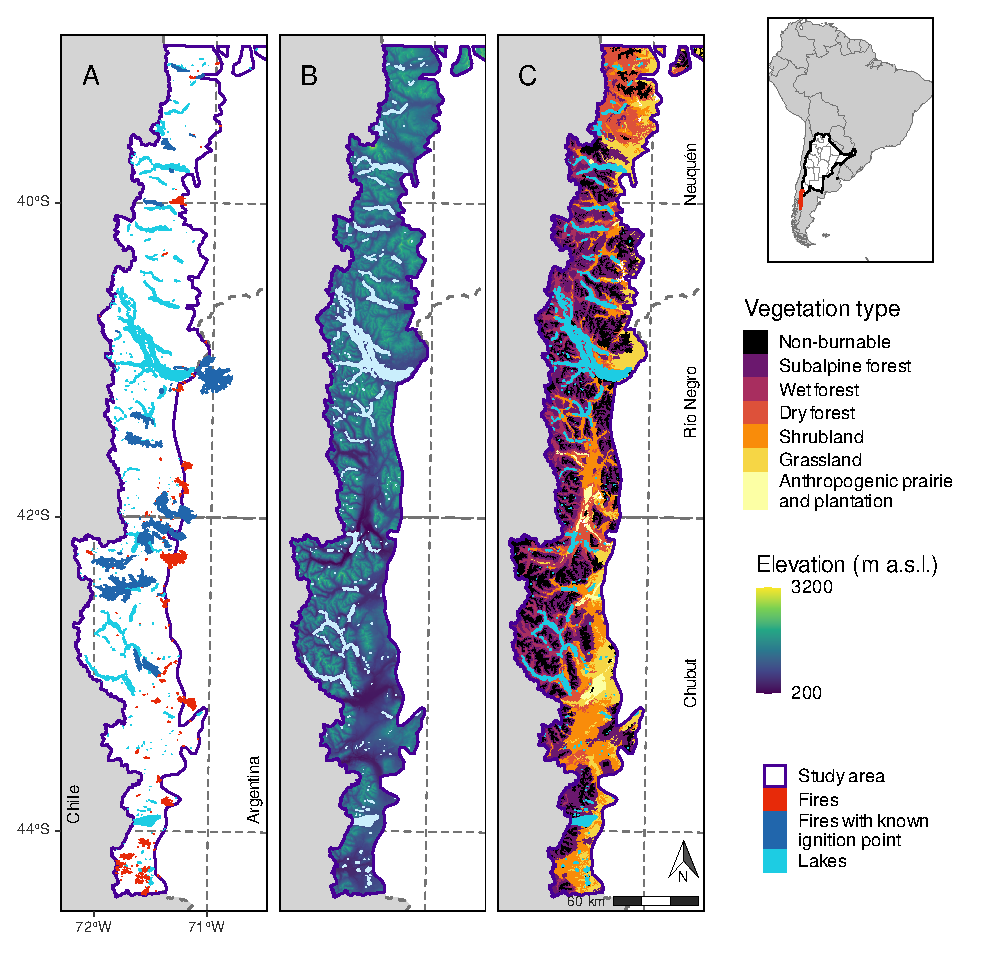
\includegraphics[width=0.95\textwidth]{fig1_study_area}
\caption{The study area, on the eastern slope of the Andes in north-western
Patagonia, Argentina. (A) The fire record: every fire $\ge$\,10\,ha mapped
between 1999 and 2022 \citep{barbera_patterns}, with the 57 fires whose
ignition point could be established (the fires the spread model was fitted
to) in the darker colour. (B) Elevation, from the 30\,m SRTM V3 digital
elevation model \citep{DEMfarr2007}. (C) Vegetation type, in the
five burnable classes the model uses plus non-burnable ground, from the merged
regional map the simulations run on \citep{lara_vegetacion_1999,mapa_ciefap}.
The dashed lines are the boundaries between the three Argentine
provinces the study area spans, named in (C).}
\label{fig:study-area}
\end{figure*}

Wet forests are dominated by the evergreen \textit{Nothofagus dombeyi} (Mirb.) Oerst.
with an understorey of the bamboo \textit{Chusquea culeou} E. Desv.; subalpine forests
of the deciduous \textit{Nothofagus pumilio} (Poepp. \& Endl.) Krasser occupy steep
slopes from $\approx$\,1200\,m\,a.s.l. to treeline; dry forests of the conifer
\textit{Austrocedrus chilensis} (D. Don) Pic.Serm. \& Bizzarri occupy low elevations at
intermediate precipitation; shrublands are formed by resprouting tall shrubs and low
trees such as \textit{Nothofagus antarctica} (G. Forst.) Oerst., \textit{Lomatia
hirsuta} (Lam.) Diels ex J.F. Macbr. and \textit{Schinus patagonicus} (Phil.) I.M.
Johnst. ex Cabrera, often with abundant \textit{C. culeou}; and grasslands correspond
mostly to the Patagonian steppe, with tussock grasses of \textit{Pappostipa} and
\textit{Festuca} and the cushion shrub \textit{Mulinum spinosum} (Cav.) Pers. Tall
forests carry a sparse, moist understorey separated from the canopy, whereas shrublands
have vertically continuous fuels with a higher proportion of dry fine dead fuel
\citep{paritsis_positive_2015, tiribelli_changes_2018, barbera_microclimate_2023}.
Fires occur from October to March, ignited by lightning and by people, mostly in warm
summers preceded by dry springs \citep{kitzberger_climatic_1997, veblen_fire_2003}.

\subsection{Data}

We used the 235 fires $\ge$\,10\,ha mapped by \citet{barbera_patterns} from Landsat
imagery at 30\,m resolution over the 24 fire seasons from July 1998 to June 2022.
Fitting the spread model requires the ignition point as well as the final perimeter,
and the ignition point could be established for 57 fires, supplied by fire management
personnel (Fig.~\ref{fig:study-area}A). The remaining 178 fires informed the parameters that
control simulated fire size. The model uses five groups of predictors, all resolved
to the 30\,m grid:

\begin{itemize}
\item \textbf{Vegetation type}, in five classes (wet forest, subalpine forest, dry
forest, shrubland, grassland), reclassified from the regional forest and land-cover map
of \citet{mapa_ciefap}; areas burned before that map was produced were patched with the
map of \citet{lara_vegetacion_1999}.

\item \textbf{NDVI} (Normalised Difference Vegetation Index), averaged over all
available Landsat images from December to March of the summer preceding each fire
season, as a proxy for productivity and fuel load.

\item \textbf{Elevation, slope and aspect}, from the 30\,m SRTM V3 digital elevation
model \citep{DEMfarr2007}. From aspect we computed \textit{northness} as its cosine,
which is 1 on north-facing and $-1$ on south-facing slopes.

\item \textbf{Wind direction and speed}. Lacking meteorological data with adequate
coverage, and with uncertain spread dates for many fires, we assumed that wind does not
change during a fire, and generated 30\,m direction and speed fields with WindNinja
\citep{forthofer2007windNinja} from a regional direction taken from the ERA5 reanalysis
\citep{hersbach2020era5} and a fixed regional speed (Section~1 of the Supplementary
material). A fire-level coefficient absorbs between-fire variation in wind forcing.

\item \textbf{Atmospheric conditions}, summarised by the FWI \citep{van_wagner_development_1987}, 
which integrates relative humidity, temperature,
precipitation and wind speed into one predictor, from the ERA5-based daily product of
\citet{vitolo_era5-based_2020}. The index was standardised per pixel, so that it
represents climatic variation in time and not in space \citep{barbera_patterns}, and
accumulated over the focal fortnight and the 10 preceding ones with weights decaying
into the past (Eqn~\ref{eq:hier1}; Section~1 of the Supplementary material).
\end{itemize}

\subsection{The spread model}

\subsubsection*{Flammability indices}

To represent the effects of vegetation type, productivity and topography with few
parameters we summarised them into a \textbf{vegetation flammability index} (VFI) and a
\textbf{topographic flammability index} (TFI). Both derive from a logistic regression
of the probability that a cell burned at least once over the study period, fitted at
the regional scale to 9194 points, whose linear predictor was
split into a vegetation part (vegetation type and a unimodal function of NDVI whose
position and curvature depend on the type) and a topographic part (elevation and
northness weighted by slope, so that it vanishes on flat ground). The model, its
coefficients and the shape of both indices are given in Section~1 of the Supplementary
material. In both indices higher values mean more flammable: 
VFI is highest in shrublands and dry
forests and lowest in wet forests, and TFI decreases with elevation and increases
towards north-facing slopes.

\subsubsection*{The cellular automaton}

The spread model propagates fire from burning cells to their eight neighbours, with a
structure close to that of \citet{morales_stochastic_2015}. Cells are burning, burnable
or non-burnable; a burning cell stays burning for exactly one iteration (\textit{step}
from here on) and then becomes non-burnable, as are water and unvegetated ground. 
Simulation starts from one burning cell or more; at each
step, spread is simulated from every burning cell to each of its burnable neighbours 
as a Bernoulli trial, and it stops when the maximum number of steps is reached or no burning
cell manages to spread. Fires are assumed to occur entirely within one fortnight, so
the model is atemporal within that period, with simulation steps not explicitly 
representing a temporal unit. 
Spread $y \in \{0, 1\}$ from cell $i$ to a burnable neighbour $j$ at step $k$ is

\begin{equation}
\label{eq:datamodel}
\begin{aligned}
    y_{ijk} &\sim \ \text{Bernoulli}(\theta_{ijk}) \\
    \theta_{ijk} &= \frac{\mathbb{I}_{k \le \kappa}}{1 + \exp{(-\eta_{ij})}} \\
    \eta_{ij} &= \beta_0 + \beta_1 \, \mathrm{VFI}_j + \beta_2 \, \mathrm{TFI}_j
                 + \beta_3 \, S_{ij} + \beta_4 \, W_{ij} \\
    S_{ij} &= \sin\left[ \tan^{-1} \left( \frac{E_j - E_i}{G_{ij}} \right) \right]
              \mathbb{I}_{E_j - E_i > 0} \\
    W_{ij} &= \cos(A_{ij} - D_i) \, V_i,
\end{aligned}
\end{equation}

\noindent where $\mathbb{I}_{k \le \kappa}$ indicates whether the number of steps
$\kappa$ has been exceeded. VFI and TFI are properties of the receiving cell, whereas
$S_{ij}$ and $W_{ij}$ are \textit{directional} terms computed from the donor--receiver
pair: $E$ is elevation (m), $G_{ij}$ the distance between cell centres, $A_{ij}$ the
bearing of the donor as seen from the receiver, $D_i$ the direction the wind blows from
at the donor
and $V_i$ the wind speed there (m\,s$^{-1}$). $S_{ij}$ is the sine of the slope between
the two cells, switched off for downhill spread by its indicator, so that downhill
spread is like spread on flat ground; $W_{ij}$ equals the wind speed when the wind blows
exactly along the direction of spread, minus the wind speed when exactly against it,
and zero when perpendicular. Over the eight-cell neighbourhood, each entry giving the
value for the receiver in that position, the distances $G_{ij}$ (m) and the bearings
$A_{ij}$ (degrees) are

\[
    G =
    \begin{bmatrix}
        30 \sqrt{2} & 30 & 30 \sqrt{2} \\
        30 & \cdot & 30 \\
        30 \sqrt{2} & 30 & 30 \sqrt{2}
    \end{bmatrix}, \quad
    A =
    \begin{bmatrix}
        135 & 180 & 225 \\
        90 & \cdot & 270 \\
        45 & 0 & 315
    \end{bmatrix},
\]

\noindent with $\cdot$ marking the donor and north at the top. A wind blowing from the
south ($D_i = 180^\circ$) therefore makes $W_{ij}$ maximal for the receiver directly
north of the donor, and a receiver uphill of it is favoured through $S_{ij}$ regardless
of direction. The unknowns are the five coefficients and the number of steps, collected as
$\boldsymbol{\beta} = \{\beta_0, \beta_1, \beta_2, \beta_3, \beta_4, \kappa\}$.

\subsubsection*{Hierarchical structure}

Fire weather enters the model through the accumulated FWI, assumed constant within a
fire and taken at the ignition cell. Even so, the model remains a simple representation
of spread: wind direction and regional speed are constant within a fire, and
suppression is not represented at all.
To absorb the process variance the model does not describe, we gave the parameters
themselves a statistical model, a hierarchical (multilevel) structure, so that FWI sets
the \emph{mean} of a distribution of spread parameters rather than determining them.
Two fires with the same FWI can then differ in weather, suppression, soil moisture and
terrain particulars:

\begin{equation}
\label{eq:hier1}
\begin{aligned}
    \boldsymbol{\beta}_{ft} &= \mathbf{L} + \frac{\mathbf{U} - \mathbf{L}}{1 + \exp{(\boldsymbol{\eta}_{ft}})} \\
    \boldsymbol{\eta}_{ft} &\sim \ \text{Multivariate Normal}(\boldsymbol{\mu}_{ft}, \boldsymbol{\Sigma}) \\
    \boldsymbol{\mu}_{ft} &= \boldsymbol{\gamma}_0 + \boldsymbol{\gamma}_1 \, x_{ft} \\
    x_{ft} &= \sum_{l=0}^{10} \mathrm{FWI}_{f,t-l} \ \frac{w_l}{\sum_{j=0}^{10} w_j},
    \qquad w_l = e^{-\left(\frac{l}{\tau}\right)^2},
\end{aligned}
\end{equation}

\noindent where $\boldsymbol{\beta}_{ft}$ is the parameter vector of fire $f$, which
occurred in fortnight $t$, and $\mathbf{L}$ and $\mathbf{U}$ hold the lower and upper
bound of each parameter, so that $\boldsymbol{\beta}_{ft}$ follows a multivariate
logit-normal distribution scaled between them. Bounding the parameters simplified
estimation and made sign restrictions easy to impose: the four slope coefficients are
constrained to be positive, so that the data inform only their magnitude, and the upper
bound on the number of steps is itself estimated. The covariance matrix
$\boldsymbol{\Sigma}$ was decomposed into standard deviations and a correlation matrix,
each with its own prior. Bounds and priors are given in Section~2 of the Supplementary
material. Because the parameters have a distribution, a mapped fire can be simulated
either with the parameter vector estimated for that particular fire or with one drawn
from the distribution given its FWI; we call these \textit{fitted} and
\textit{simulated} random effects respectively.

\subsection{Parameter estimation}

The cell-to-cell spread events $y_{ijk}$ are not observed: at best the ignition point
and the final perimeter are known, and how the fire moved between them could not be
recorded. The likelihood therefore cannot be evaluated, and we used Approximate
Bayesian Computation (ABC; \citealt{beaumont2010approximate, sisson2018handbook}), as
\citet{morales_stochastic_2015} did for a similar model in this region. 
ABC replaces the likelihood with similarity, favouring parameter values that make the fires they
simulate more similar to the observed one. Similarity was measured by spatial overlap, the
number of cells burned by both fires divided by the number burned by either 
(intersection over union), and every
simulation of a mapped fire used that fire's own spatial predictors, FWI and ignition
point.

The full hierarchical model could not be sampled directly: the parameters are many,
and the ABC kernel is stochastic and varies abruptly with $\boldsymbol{\beta}$, which
makes conventional MCMC prohibitively expensive. We therefore applied what we believe is a new
strategy: the two-stage method of \citet{lunn2013fully}, driven by fire-wise ABC
posteriors. Stage 1 sampled the posterior of $\boldsymbol{\beta}_f$
separately for each of the 57 fires with a known ignition point, under a placeholder
prior uniform over $[\mathbf{L}, \mathbf{U}]$, with adaptive ABC sequential Monte Carlo
\citep{delmoral2012adaptive} whose particles move by Metropolis steps with a
differential-evolution proposal \citep{terbraak2006markov}. Stage 2 combined those
samples into the hierarchical model with a Metropolis-within-Gibbs sampler: each fire's
stage-1 sample served as the proposal for its own random effects, with the placeholder
prior discounted in the acceptance ratio, while most hyperparameters were drawn from
their conditional distributions in conjugate Gibbs steps. Splitting the model this way
confines the fire simulator to stage 1.

The 57 fires with a known ignition point are larger, on average, than the mapped
record as a whole, which would bias the parameters that govern simulated fire size,
the number of steps $\kappa_f$ and its hyperparameters. To correct that bias we fitted,
jointly with the rest of the model, an auxiliary regression of burned area on the
number of steps, through which the steps of the 178 fires with an unknown ignition point,
which cannot be simulated, are inferred from their area. Section~2 of the Supplementary
material gives the full specification of both stages, the auxiliary regression and the
convergence diagnostics. The fire simulator is written in C\texttt{++} and distributed
as the R package \texttt{FireSpread} v1.4 \citep{firespread} through \texttt{Rcpp}
v1.1.0 \citep{Rcpp}; all fitting and analysis was done in R 4.5.3 \citep{R}, with
\texttt{terra} v1.8.70 \citep{terra} for spatial data management.

\subsection{Validation}

Classical train/test validation is not appropriate here, as our aim was not
to develop a spread model to predict the spread of individual fires
(see Section~3 of the Supplementary material), and burn-probability models are
conventionally judged on the emergent properties of the regime they generate rather
than on point predictions of individual fires \citep{parisien2020commentary}. We
therefore validated the model in the pattern-oriented sense \citep{grimm2005pattern,
hartig2011statistical}, asking whether statistical patterns emerging from many
simulated fires match those of the observed record, using patterns the fitting
procedure did not target. Two exercises did this at two scales, and neither
recalibrated any parameter.

The first re-simulated the mapped fires. For each of the 57 fires with a known ignition
point we simulated 2000 fires from its own ignition cell and landscape under its fitted
random effects, and 2000 more under simulated random effects drawn from the population
distribution at its FWI. Each simulated fire was reduced to its spatial overlap with
the observed one, its burned area overall and within each vegetation class, its
compactness ($4\pi \times$ area / perimeter$^2$) and the deviation of its principal
axis from the fire's own wind axis. Each statistic was then turned into a scaled
quantile residual \citep{dunn1996randomized}, the position of the observed value among
the 2000 simulated ones, computed with \texttt{DHARMa} v0.4.7 \citep{DHARMa}: uniform
on $(0, 1)$ if the model is calibrated for that statistic.

The second simulated many fires over the whole study area, 
not using the fitted random effect, but simulated ones. 
Every simulated fire took an FWI value
resampled from the mapped record, a draw from the joint posterior of the
hyperparameters, random effects drawn afresh for a \emph{new} fire, and an ignition cell
at random from the burnable landscape.
After running 200\,000 fires and discarding those below 10\,ha 
(same threshold as in the mapped record)
we obtained 87\,309 simulated fires to compare against the 235 observed ones. 
We compared these with the observed
record in the distribution of fire size and in shape, measured as compactness and as the
deviation of a fire's principal axis from the dominant regional wind axis. Both need
only a rasterised perimeter, so the observed reference is every mapped fire in the
record, not only the 57 with a known ignition point. Because shape depends strongly on
size, and size is itself being tested, the shape comparisons were made conditionally on
burned area as well as marginally, and repeated conditionally on FWI, which tests the
model's most distinctive structural claim: that the parameters of spread shift with
fire weather. Section~3 of the Supplementary material explains both validation
routines fully.

\section{Results}

\subsection{What drives spread probability}

Spread probability responded most strongly to the two directional terms. At the mean
FWI of the mapped fires, and holding every other predictor at its mean, spread
probability rose from 0.06 on flat ground to 0.79 towards a neighbour 45$^\circ$ uphill,
and from 0.01 for a neighbour directly upwind to 0.76 for one directly downwind
(Fig.~\ref{fig:curves}). The two flammability indices moved it far less over their
observed ranges: from 0.03 to 0.25 across VFI and from 0.04 to 0.23 across TFI.
Decomposed into the raw predictors they are built from (Fig.~S2), the strongest single gradient is
elevation, with spread probability falling from 0.25 at 500\,m\,a.s.l.\ to 0.08 at
1200\,m.

Fire weather shifted the curves, but not all of them and not equally. Raising the FWI
anomaly from $-0.60$ to 2.38 (the 2.5th and 97.5th percentiles of the mapped fires)
lifted downwind spread probability from 0.59 to 0.88 and nearly doubled spread
probability on flat ground, from 0.055 to 0.100, while leaving the top of the slope
curve unchanged (0.80 to 0.78) and the probability of spreading directly upwind
negligible throughout (0.014 to 0.009) (Fig.~\ref{fig:curves}).

\subsection{Between-fire variation and its relation to fire weather}

The spread parameters varied greatly among fires, and FWI explained only part of that
variation (Fig.~\ref{fig:params}). The number of steps $\kappa$ increased with FWI with
complete certainty (posterior probability of a positive population slope, $P = 1.00$),
and the wind coefficient $\beta_4$ increased too ($P = 0.92$). The other four were
indistinguishable from flat: $P = 0.74$ for the intercept, 0.55 for TFI, 0.34 for slope
and 0.23 for VFI. Fire weather therefore acts mainly on how far a fire runs and on how
strongly wind steers it, with no clear effect on how the local landscape modulates spread.

Across fires the parameters were correlated (Fig.~S3). The wind coefficient was
negatively correlated with the VFI coefficient (posterior mean correlation $-0.45$),
so that a strongly wind-driven fire was one whose spread depended little on vegetation,
and with the slope coefficient ($-0.18$), so that fires tend to be dominated by slope or
by wind rather than by both. It was positively correlated with the number of steps
(0.25): windier fires ran further.

Because the logistic link is nonlinear, a coefficient that does not respond to FWI can
still have a weather-dependent effect on the probability. At the lowest FWI, mean spread
probability ranged from 50\,\% in wet forest through 59\,\% in subalpine forest, 65\,\%
in grassland and 69\,\% in dry forest to 72\,\% in shrubland; at the highest FWI every
type rose, to 71, 79, 83, 86 and 87\,\% respectively (Fig.~\ref{fig:vegeffect}B). The
vegetation effect (the mean absolute deviation among the five types) fell from 6.8
to 4.9 percentage points, with posterior probability 0.79 that it declines
(Fig.~\ref{fig:vegeffect}A). Severe fire weather thus narrows the differences among
vegetation types without erasing them, and it narrows them by lifting every type rather
than by holding the flammable ones back.

\subsection{Validation: re-simulating the mapped fires}

Given each fire's own fitted random effects, the simulator reproduced the mapped fires
reasonably well: the median spatial overlap over the 57 fires was 0.53 (range
0.15--0.83; Fig.~S4) and the median over fires of the mean simulated-to-observed size
ratio was 1.09, with
55 of 57 fires within a factor of two (Fig.~S5). Under simulated random effects 
the median overlap shrank to 0.11 (range 0.03--0.24), and median size ratio was 1.51, 
with only 28 of 57 fires within a factor of two. The per-cell picture is the same
(Fig.~\ref{fig:bp}): with fitted random effects the high-probability region is close
to the fire perimeter, whereas with simulated random effects probability spreads
out around the ignition point and the perimeter is no longer traced.
The quantile residuals also quantify a mismatch in size distribution. 
(Fig.~\ref{fig:dharma}, Table~\ref{tab:dharma}). Each residual is the quantile at which
a fire's observed value falls among its own simulations. These residuals have a uniform
distribution in (0, 1) if the model is calibrated, and their average across fires should be near 0.5. Lower means
the model burns too much, higher too little. For burned area under fitted random
effects the observed fires show a mean residual of 0.373, so the model burns too much. 
Under simulated random
effects the residuals moved the other way (mean 0.686), because that
distribution widens so much that most simulations fall short of the observed fire even
though their mean exceeds it: the quotient above averages simulations, this residual
ranks them. This mean above 0.5 under simulated random effects is probably the 178 
smaller fires (those whose ignition point is unknown) pulling the steps distribution to
the small side.

The two shape statistics behaved differently.
Under simulated random effects the mean compactness residual was 0.163, with
96\,\% of observed fires less compact than the median simulation of their own fire, and
the mean wind-axis residual was 0.245, with 90\,\% of observed fires better aligned with
their own wind than the median simulation. Under fitted random effects both are closer
to calibration (0.429 and 0.325), as expected of a fit diagnostic against an
out-of-sample one, but the sign is the same: real fires are less compact and better
aligned with the wind than the model makes them. Every panel departs from uniformity
in both modes.

\subsection{Validation: the regional simulation}

Over the whole study area, the 87\,309 simulated fires were larger than the mapped
record, and uniformly so rather than in one tail: the quantile--quantile relation sits
below the 1:1 line over the entire range (Fig.~\ref{fig:validation}A), the
Kolmogorov--Smirnov statistic is $D = 0.192$ ($P = 3.7 \times 10^{-8}$), and the offset
is a factor of about two to three through the middle of the distribution: median 155
against 58\,ha, 75th percentile 902 against 321\,ha, 95th percentile 9959 against
3249\,ha. The response of size to fire weather, in contrast, matched: across quartiles
of FWI the observed median area rose from 40 to 278\,ha and the simulated median from
56 to 408\,ha (Fig.~\ref{fig:validation}B), the same relative increase carrying the
same offset.

Shape did not match at any size (Table~\ref{tab:shape}). Simulated fires were rounder
than observed ones in every size class: median compactness 0.34 against 0.24 below
100\,ha, 0.27 against 0.10 between 100 and 1000\,ha, and 0.08 against 0.03 above
1000\,ha. The median deviation of a fire's
principal axis from the regional wind axis was 31, 32 and 20$^\circ$ for observed fires
in the three size classes, against 45$^\circ$ under random orientation, but 55, 59 and
60$^\circ$ for simulated ones: the observed record is wind-aligned, most strongly among
the largest fires, whereas the simulated set is if anything oriented slightly across the
wind. Conditioning on FWI does not change these patterns (Fig.~\ref{fig:validation}B):
observed compactness falls with FWI and simulated compactness falls in parallel,
roughly 0.15 higher throughout, and the deviation from the wind axis is flat in both,
near 35$^\circ$ observed and 50$^\circ$ simulated.

%TC:ignore
\begin{table*}[tp]
\tbl{Calibration of the model against the 57 fires with a known ignition point
(Fig.~\ref{fig:dharma}). For each statistic and each way of setting the
random effects, the mean scaled quantile residual over fires (0.5 under perfect
calibration), the fraction of fires whose observed value falls below the median of its
own 2000 simulations (0.5 under perfect calibration) and the Kolmogorov--Smirnov
statistic against the uniform distribution. $n$ is the number of fires entering the
panel; a fire is excluded from a vegetation class if fewer than 30 cells of that class
were available to burn in its landscape.\label{tab:dharma}}{%
\begin{tabular*}{\textwidth}{@{\extracolsep{\fill}}lrrrrrrr}
\toprule
& & \multicolumn{3}{c}{Fitted random effects} & \multicolumn{3}{c}{Simulated random effects} \\
\cmidrule(lr){3-5} \cmidrule(lr){6-8}
Statistic & $n$ & Residual & Frac. below & $D$ & Residual & Frac. below & $D$ \\
\midrule
Burned area, all types    & 57 & 0.373 & 0.65 & 0.25 & 0.686 & 0.19 & 0.34 \\
\quad Wet forest          & 49 & 0.446 & 0.51 & 0.29 & 0.649 & 0.27 & 0.31 \\
\quad Subalpine forest    & 46 & 0.534 & 0.41 & 0.22 & 0.709 & 0.13 & 0.39 \\
\quad Dry forest          & 49 & 0.485 & 0.53 & 0.26 & 0.652 & 0.27 & 0.28 \\
\quad Shrubland           & 57 & 0.291 & 0.75 & 0.42 & 0.649 & 0.23 & 0.28 \\
\quad Grassland           & 55 & 0.231 & 0.80 & 0.52 & 0.596 & 0.35 & 0.22 \\
Compactness               & 57 & 0.429 & 0.56 & 0.35 & 0.163 & 0.96 & 0.52 \\
Deviation from wind axis  & 57 & 0.325 & 0.70 & 0.43 & 0.245 & 0.90 & 0.47 \\
\bottomrule
\end{tabular*}}{}
\end{table*}

\begin{table*}[tp]
\tbl{Median shape of observed and simulated fires by size class, over the whole study
area: the mapped fire perimeters against the 87\,309 simulated fires. Compactness is
$4\pi \times$ area / perimeter$^2$, larger for rounder fires. Deviation from the wind axis
is the angle between a fire's principal axis and the regional wind direction, folded into
0--90$^\circ$; a set of randomly oriented fires would have a median of 45$^\circ$ and a
fraction within 30$^\circ$ of the axis of 0.33.\label{tab:shape}}{%
\begin{tabular*}{\textwidth}{@{\extracolsep{\fill}}llrrr}
\toprule
& & $<$ 100 ha & 100--1000 ha & $>$ 1000 ha \\
\midrule
Number of fires & observed   & 146 & 59 & 36 \\
Compactness & observed       & 0.24 & 0.10 & 0.03 \\
            & simulated      & 0.34 & 0.27 & 0.08 \\
Deviation from wind axis ($^\circ$) & observed  & 31 & 32 & 20 \\
                                    & simulated & 55 & 59 & 60 \\
Fraction within 30$^\circ$ of the axis & observed  & 0.48 & 0.46 & 0.72 \\
                                       & simulated & 0.29 & 0.27 & 0.26 \\
\bottomrule
\end{tabular*}}{}
\end{table*}
%TC:endignore

\begin{figure*}[tp]
\centering
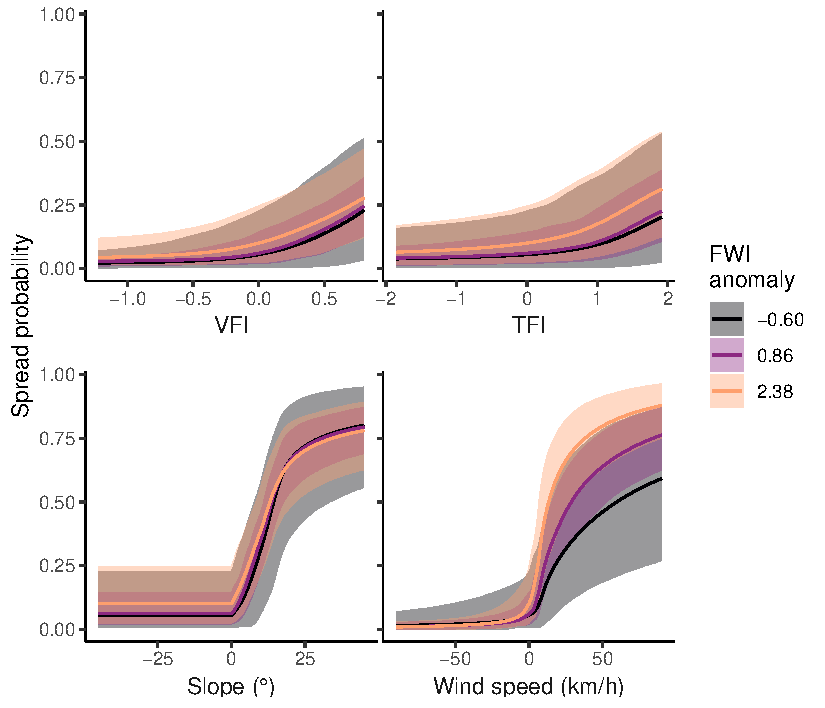
\includegraphics[width=0.75\textwidth]{fig2_spread_curves}
\caption{Spread probability as a function of each predictor, at three contrasting values
of accumulated FWI: the mean and the 2.5th and 97.5th percentiles of the mapped fires,
shown on the original anomaly scale. Each curve is the average over the estimated
distribution of parameters, obtained by simulation; lines and bands are the mean and the
95\,\% credible interval of the posterior. VFI, vegetation flammability index; TFI,
topographic flammability index (Section~1 of the Supplementary material); both are
dimensionless, and higher values mean more flammable. Slope and wind speed are signed:
positive values are uphill and downwind. The remaining predictors are held at their
means.}
\label{fig:curves}
\end{figure*}

\begin{figure*}[tp]
\centering
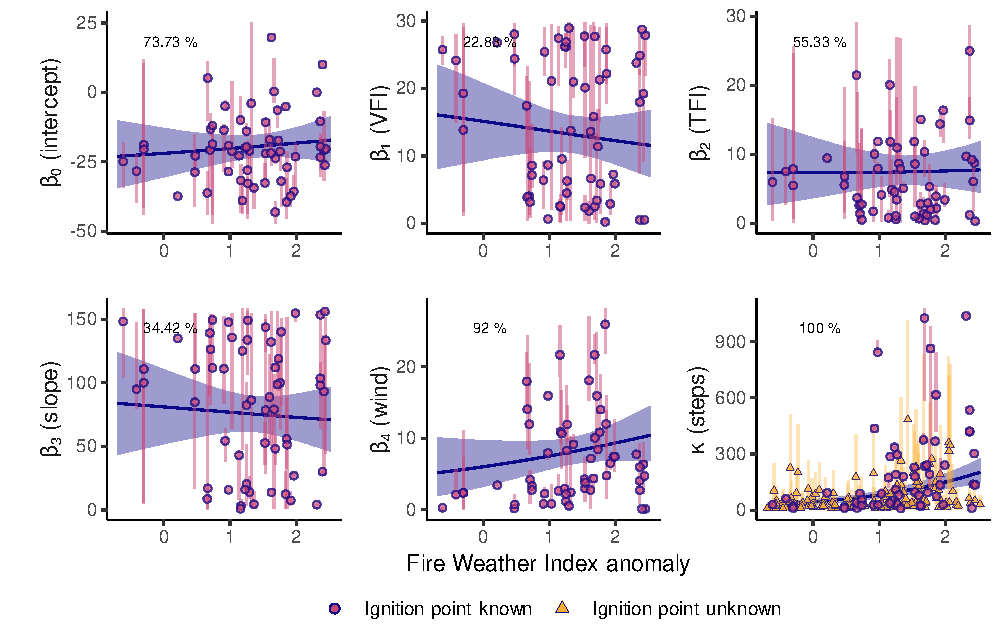
\includegraphics[width=1.0\textwidth]{fig3_params_fwi_v2}
\caption{The six spread parameters as a function of accumulated FWI. Lines and bands are
the mean and the 95\,\% credible interval of the population mean; points and vertical
lines are the parameter estimated for each of the 57 fires with a known ignition point,
as a posterior mean and 95\,\% credible interval. The percentage in each panel is the
posterior probability that the population mean increases with FWI (0\,\% is certainty of
a negative effect, 50\,\% complete uncertainty about the sign, 100\,\% certainty of a
positive one). $\kappa$ is the maximum number of simulation steps
(Eqn~\ref{eq:datamodel}).}
\label{fig:params}
\end{figure*}

\begin{figure*}[tp]
\centering
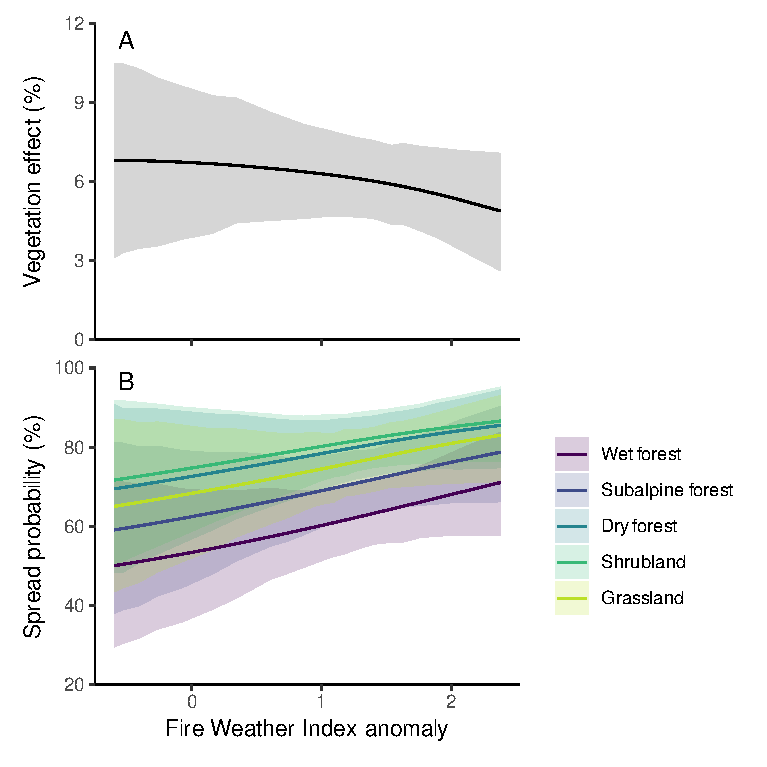
\includegraphics[width=0.58\textwidth]{fig4_vegetation_effect}
\caption{(A) The effect of vegetation type on spread probability as a function of
accumulated FWI, computed as the mean absolute deviation among the five types' spread
probabilities shown in (B). (B) Spread probability by vegetation type. To make the types
comparable, elevation is fixed at 900\,m\,a.s.l.\ and aspect at 90$^\circ$ (northness
$= 0$), and the prediction is marginalised over the distribution of NDVI, slope and wind
speed in the study area and over the estimated distribution of parameters. Lines and
bands are the mean and the 95\,\% credible interval of the posterior.}
\label{fig:vegeffect}
\end{figure*}

\begin{figure*}[tp]
\centering
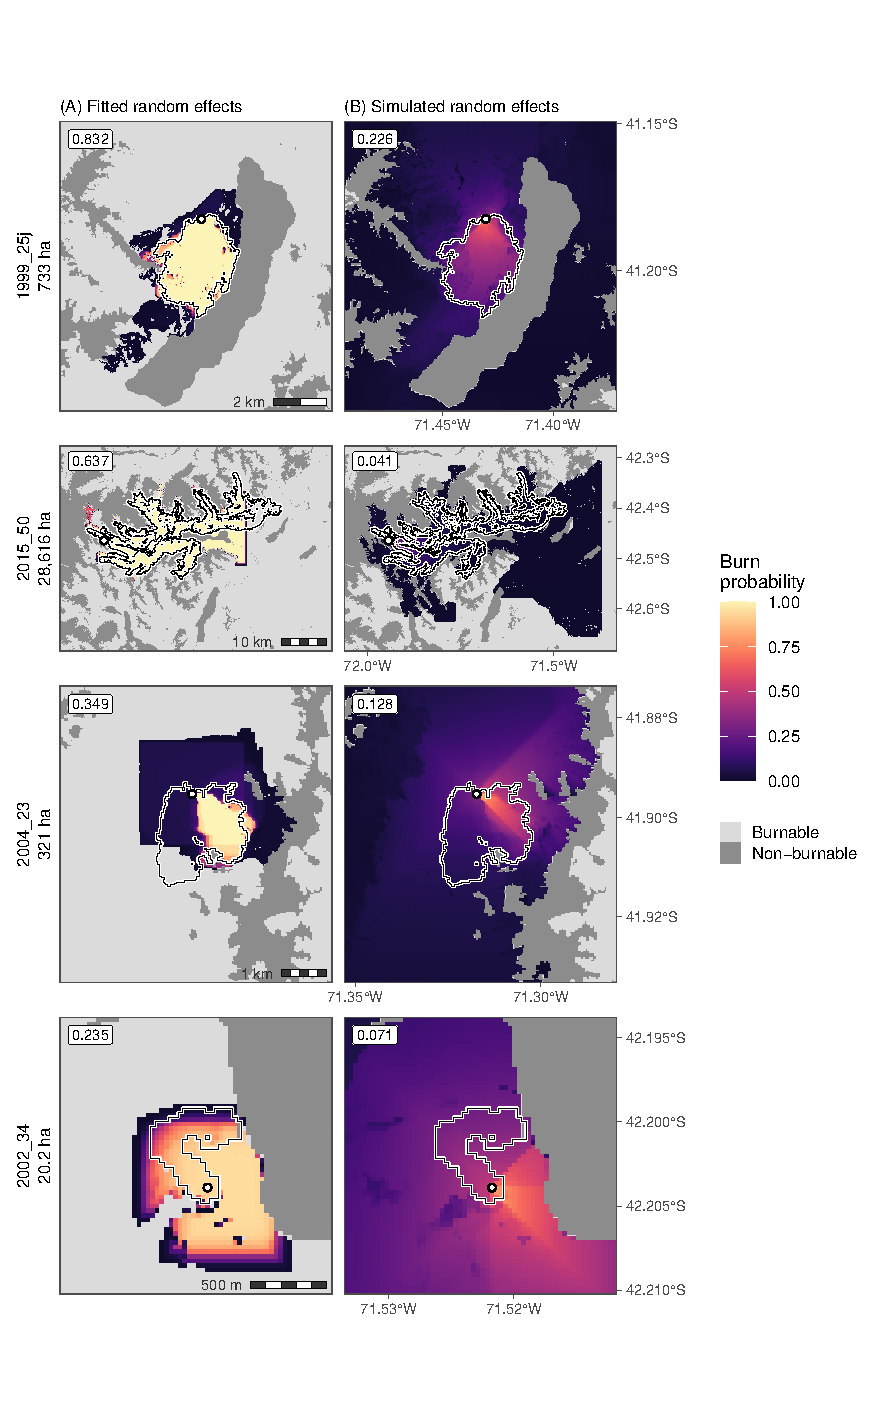
\includegraphics[width=0.65\textwidth]{fig5_burn_probability}
\caption{Per-cell burn probability for four of the fires with a known ignition point,
from 2000 simulations under the fire's own fitted random effects (A) and 2000 under
random effects drawn afresh from the estimated distribution (B). The four fires span three
orders of magnitude in size and a gradient of goodness of fit. The observed perimeter is
outlined in white and the ignition point is the white dot; the base map distinguishes
burnable from non-burnable ground. The number in each panel is the mean spatial overlap
between the simulated and the observed fire over the 2000
simulations. The blocky outer boundary of the probability surface is the limit set by the
number of steps $\kappa$, not a landscape edge.}
\label{fig:bp}
\end{figure*}

\begin{figure*}[tp]
\centering
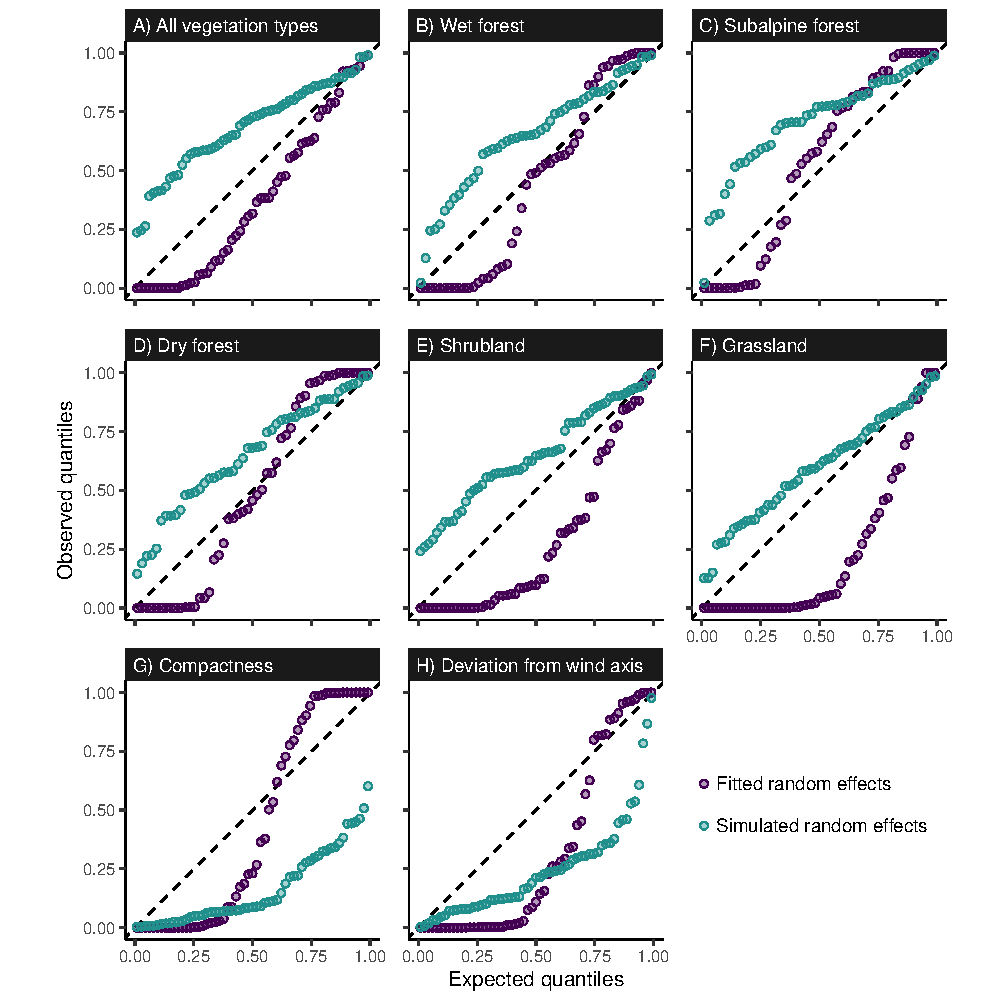
\includegraphics[width=0.85\textwidth]{fig6_dharma_metrics}
\caption{Scaled quantile residuals for the 57 fires with a known ignition point, against
the expected uniform quantiles. Each point is one fire: the position of its observed
value within the 2000 values simulated for that same fire from that same ignition point.
Points on the 1:1 line indicate a calibrated model, points below it that the model
simulates too much of the quantity and points above it too little. (A--F) burned area,
overall and within each vegetation class; (G) compactness; (H) the deviation of the
fire's principal axis from its own wind axis. Colours distinguish the two ways of setting
the random effects. Summary statistics are in Table~\ref{tab:dharma}.}
\label{fig:dharma}
\end{figure*}

\begin{figure*}[tp]
\centering
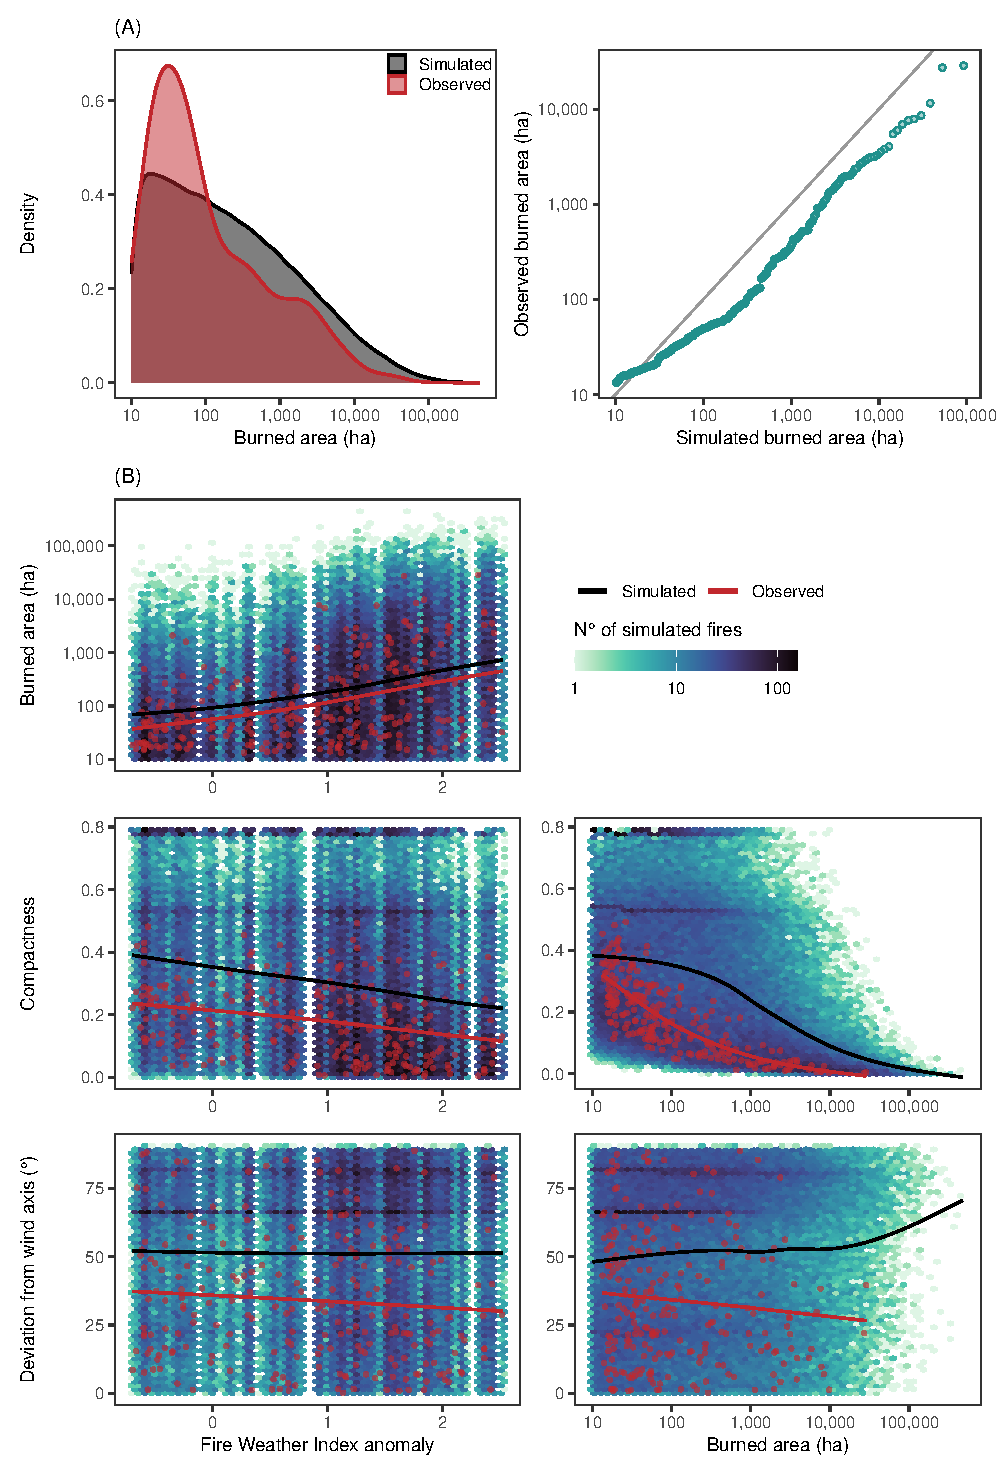
\includegraphics[width=0.68\textwidth]{fig7_validation}
\caption{The 87\,309 fires simulated over the whole study area against the mapped record.
(A) The distribution of burned area, as overlaid densities and as a quantile--quantile
plot; the grey line is the 1:1 relation. (B) Burned area, compactness and the deviation
of the fire's principal axis from the regional wind axis, each conditioned on FWI (left)
and on burned area (right). Simulated fires are shown as a hexagonal-bin density on a
logarithmic count scale and observed fires as points, with a generalised additive
smoother through each. FWI is on the same anomaly scale as
Figs.~\ref{fig:curves}--\ref{fig:vegeffect}. The vertical striping of the left-hand
panels is real: FWI was resampled from the values of the mapped record, so the simulated
set takes only those values.}
\label{fig:validation}
\end{figure*}

\section{Discussion}

Fitted to nothing more than final perimeters and ignition points, the model recovered
the general structure of fire behaviour that physical models encode. Spread probability
responded above all to the two directional terms, wind and slope, with vegetation and
topography as secondary controls (Fig.~\ref{fig:curves}), which is the ordering of the
Rothermel equations \citep{rothermel_mathematical_1972} and of the previous model for
the region \citep{morales_stochastic_2015}. Two features of the between-fire variation
are also realistic. The wind and slope coefficients were negatively correlated, so a fire
is driven by one factor or the other rather than by both at once. That is also how
wildfires are usually classified from their spread pattern: wind-driven fires follow the
direction of a strong regional wind, whereas topographic fires are steered by slope and
by the local winds the terrain itself generates \citep{lecina_extreme_2014}.
And the wind coefficient was positively correlated with the number of
steps, so that windier fires ran further; the correlation also keeps the simulator from
producing fires that spread in every direction for many steps, which would be enormous.
That fire weather acted on reach and on the wind effect, and not on the vegetation and
topography terms, is coherent with the FWI being an increasing function of wind speed
as well as of temperature, humidity and rain.

That last result has an ecological reading. Many studies report that bottom-up
controls attenuate under extreme fire weather: fuel types or topographic positions that
normally limit spread stop being effective barriers \citep{Podur2009, Parks2015,
Collins2019, jones_extreme_2023}. We found instead that the effect of vegetation, though
secondary, persisted at the highest FWI in the record: severe weather lifted spread
probability in every type without closing the gap between closed forests and shrublands
(Fig.~\ref{fig:vegeffect}). Tall closed forests carry moister fuel, less vertical
continuity and more coarse fuel acting as a heat sink \citep{zylstra_biophysical_2016,
barbera_microclimate_2023, tiribelli_changes_2018}, and although every type can burn when the atmosphere
allows it, spread through them appears to remain slower. This suggests that maintaining
tall closed canopies could slow spread across the landscape even in severe seasons.

\subsection*{Two meanings of the random effects}

The model reproduces a mapped fire well when given that fire's own random effects and
poorly when given random effects drawn from the population. That gap is not a failure
of the fit; it is a measurement of how much of a fire's behaviour is carried by the
things the random effects absorb. Within a fortnight the model sees one wind direction,
one regional wind speed, one FWI value and no suppression at all, so a fire that was
fanned by an unusually strong wind, or stopped early by rain or by fire crews, can only
be represented through its own random effects. Simulating with a fresh draw is
simulating a different fire under the same weather index and on the same landscape, and
the drop in overlap from 0.53 to 0.11 measures the width of that distribution rather
than an error. A regime simulator needs the second mode, generating plausible fires
rather than retrodicting particular ones, which is why the record-wide experiment is
the test that matters the most for the model's intended use. Note too that a simulated fire
stops either because propagation failed at every edge cell or because the step budget
$\kappa$ ran out; $\kappa$ is a lumped stand-in for everything that ends a fire in
time, a weather change, rain or successful suppression.

\subsection*{Problems with the spread geometry}

The clearest mismatch in both validation exercises is shape, and it reveals a structural problem. 
In the automaton the spread \emph{rate} is isotropic: the front advances at most one cell per step
in every direction, and the wind term changes only \emph{whether} a neighbour ignites, never
how fast the front reaches it. Under a strong wind the downwind cell and the two diagonals
45$^\circ$ off the wind axis, which still take 71\,\% of the wind term, all saturate at a
spread probability near 1, so the flanks advance as fast as the head: simulated fires in
flat, homogeneous fuel make a funnel widening downwind, never the narrow, cigar-shaped run
of a wind-driven fire. This also explains the size mismatch, since for the same step budget
($\kappa$) a compact fire burns far more area than an elongated one.

The automaton can only produce elongated fires when spread probability is low enough 
that the effective front speed itself differs between
downwind and lateral directions (as in \citealt{morales_stochastic_2015}). Consistent with
this, the shape mismatch is carried mostly by the fires that used up their step budget.
This hard limit confines them to a square around 
their ignition cell and clips the downwind axis first,
leaving them rounder and turned across the wind. Fires that ended because propagation failed
at every edge cell are closer to the mapped record (Section~5 of the Supplementary material).
But spread under low probability leaves many unburned islands within
them, which would overestimate the regeneration capacity of seeder species in simulations of
post-fire vegetation transitions. The model can make fires elongated or large, but not both.

The remedy is a different geometry. The eight-neighbour contagion automaton, adopted from
\citet{morales_stochastic_2015} because it was cheap and required no rate of spread, has no
notion of travel time, so the shape of a simulated fire is set by the grid rather than by the
wind. Elliptical growth models instead treat every point on the front as the source of an
ellipse whose elongation is a function of wind speed \citep{van_wagner_simple_1969,
anderson_predicting_1983, richards_elliptical_1990}, and two efficient implementations exist:
minimum travel time \citep{finney_fire_2002}, which solves fire arrival times as a
shortest-path problem on the grid, and cell-based elliptical automata such as Cell2Fire
\citep{pais_cell2fire_2021}. Both assume weather constant during a run, which our fortnightly
formulation assumes anyway, and both are cheap enough for the thousands of simulations a
regime simulator requires. What makes them data-hungry is not the geometry but the
rate-of-spread equations that feed it, which need fuel models; those could be replaced by an
empirical rate of spread: a base rate defined as a function of VFI, TFI
and FWI multiplied by a wind response, with the length-to-breadth ratio taken from
\citet{anderson_predicting_1983}. Such a model would have no more parameters than ours, and
the fitting approach developed here applies to it unchanged.

\subsection*{Further improvement using fire progression data}

The assumption that fires burn under constant weather within a temporal unit (here a
fortnight) is coarse, but it is what allows the model to be fitted with the data
available. With better data the unit could be shrunk to a day, half a day or a quarter of a day,
and datasets of fire progression that did not exist when this record was compiled now
make that possible. GlobFire delimits fire events and their daily burned area worldwide
from the 500\,m MODIS product \citep{artes_global_2019}, and the same approach has been
applied across the United States \citep{balch_fired_2020}. Regional efforts reach finer
detail at a much higher cost: half-daily perimeters and active fronts tracked from VIIRS
across California \citep{chen_california_2022}, and a rate of spread per burning period
reconstructed for 80 Portuguese fires from satellite, airborne and ground records
\citep{benali_portuguese_2023}.

All of them miss small fires: at 375--500\,m resolution they resolve only fires of tens
of hectares or more, whereas most of the record here is below 100\,ha
(Table~\ref{tab:shape}). Hence, a model fitted to progression data alone would inherit the
size distribution of large fires. Informing different parameters with different datasets,
as we did through the area regression, avoids that. The spread functions are fitted from the fires
with progression data, and the parameters that govern fire size, like our $\kappa$, from
the final perimeters of the whole record. Mapping the daily advance of small fires is currently
within reach too: PlanetScope delivers near-daily 3\,m images and resolves burns too
small and fragmented for coarser sensors \citep{martins_deep_2022}.

\subsection*{What the hierarchical structure makes possible}

A model that explains more of the between-fire variation, through daily weather and a
better geometry, will leave less to the random effects, but not nothing. Suppression is
the clearest case: it ends many fires early, it is recorded for few, and it is not a
function of any mapped covariate. Here it is lumped into $\kappa$. It could instead be a latent
variable per fire controlling initial spread, informed by suppression records where they
exist and estimated where they do not, and simulated from its own distribution, so the
simulator produces the mix of small and large fires the record shows. The same logic extends to the inputs. Weather and
ignition point were treated as known here, corrected by hand where a fire's shape
contradicted the reanalysis, but for poorly documented fires the spread date and the
ignition point could be parameters, given informative priors and bounded by the
satellite detections that constrain both, and estimated jointly with the spread
parameters.

Both extensions depend on the structure being fittable. Hierarchical models have
been fitted by ABC before, but in the published schemes the simulator runs inside the
sampler \citep{bazin2010likelihood, turner2014hierarchical, clarte2021componentwise}, and
the two-stage scheme of \citet{lunn2013fully}, used in ecology to fit hierarchical movement
models \citep{hooten2016hierarchical}, assumes a likelihood in its first stage. Using
fire-wise ABC posteriors as its proposal pools joins the two: the hierarchical model is
fitted without running the simulator again, so the costly step is done once per fire, and
new fires can be added without refitting the old ones.

\subsection*{Contributions}

The spread engine used here should be replaced, but the approach built around it is valuable.
Four of its strategies are useful for developing the spread component
of fire regime simulators where fire behaviour is poorly documented. 
The first is simplifying the process to what the data can inform, 
one event per fire under one wind and one weather value. 
The second is fitting different parts of the model from different data: 
the whole model from the fires with a known ignition point, by simulation, 
and the parameters that govern size from the whole record, by matching size. 
The third is the hierarchical structure, which turns
the unobserved into a distribution that can be simulated and linked to variables that
we can measure (e.g., coarse weather, fire suppression resources).
The fourth is the estimation method, which we believe is new: fire-wise ABC posteriors as
the proposal pools of a two-stage fit. It accommodates the extensions above without change, since stage 1 samples whatever is fire-specific and stage 2
never runs the simulator. All of them could be adopted with a better spread engine.

\section{Conclusion}

A six-parameter spread model fitted to final perimeters recovered the dominant
controls of fire behaviour in north-western Patagonia: wind and slope above vegetation
and topography, together with a realistic response of fire size to fire weather and a
vegetation effect that persists under severe weather. Its contagion geometry cannot
produce the elongated, wind-aligned fires the record contains, and this one structural
limit explains both the shape mismatch and the size overshoot of the simulated regime.
The remedy is a change of engine, not of approach: an elliptical spread geometry driven
by an empirical rate of spread would keep the model as cheap and as frugal with data as
this one. The hierarchical structure, the combination of data sources and the two-stage
ABC fit developed here apply to such a model unchanged, and are the parts of this work
we expect to be of use wherever fire regimes must be simulated from a record of
perimeters alone.

%==============================================================================
%  END OF THE 6000-WORD BUDGET.
%==============================================================================
%TC:ignore

%------------------------------------------------------------------------------
% ONLINE SUMMARY, 50-80 words, exactly three sentences, for non-experts:
%   1. engage the reader / why this area matters
%   2. the problem addressed + the main discovery
%   3. the bigger picture (implications, impact)
% Optional image alongside it (needs permission + photographer credit).
%------------------------------------------------------------------------------
\begin{onlinesummarytext}[Online Summary Text:]
Fire activity is increasing in the Patagonian forests, and
simulation models are the only way to explore what the landscape may look like in
decades to come. We built and tested a simple fire spread model that can be fitted
from mapped fire perimeters and ignition points alone. The model 
captures the main characteristics of fire spread in this region,
but not the elongated shape of wind-driven fires.
The fitting approach carries over to better spread models, offering a cheap way to
simulate fire regimes in regions where fire behaviour is poorly documented.
\end{onlinesummarytext}

\section{Supplementary material}

Supplementary material is available online. Section~1 details the wind field, the
accumulated Fire Weather Index and the flammability indices (Table~S1, Fig.~S1);
Section~2 the priors and the two-stage estimation procedure; Section~3 the validation
statistics; Section~4 the vegetation comparison behind Fig.~\ref{fig:vegeffect}; and
Section~5 the extended results, with a further analysis of fire shape by what brought
each simulated fire to a stop (Table~S2, Fig.~S6).

\section{Acknowledgements}

We thank Sandro Lobos and Jorge Bonansea (Brigada de Puerto Patriada, Servicio Provincial
de Manejo del Fuego, Chubut), who located the ignition points of many of the fires used to
fit the spread model.

%------------------------------------------------------------------------------
% REFERENCES, Harvard (CSIRO). BibTeX with the class's own style file.
% natbib is loaded by the class in authoryear mode:
%   \citep{key}     -> (Smith 2024)
%   \citet{key}     -> Smith (2024)
%   \citep[p.~6]{k} -> (Smith 2024, p. 6)
%   several keys in ONE \citep{a,b} -> chronological order, ';' separated
% Multiple keys in one \citep must be listed in CHRONOLOGICAL order, natbib does
% not sort them for us, the class loads it without the `sort' option.
% Reminder: full journal names (never abbreviated), DOIs where available,
% >= 3 author names then et al., never ellipses.
% ijwf.bst is our patched copy of the CSIRO samplebib.bst, see README.md here.
%------------------------------------------------------------------------------
\bibliographystyle{ijwf}
\bibliography{references}

%------------------------------------------------------------------------------
% COMPULSORY AUTHOR STATEMENTS
%------------------------------------------------------------------------------
% The class builds framedbox as an mdframed inside a full-width `strip'. If the box
% has to be split across a page, mdframed's split loop sends pdflatex into a
% SEGMENTATION FAULT (exit 139, log truncated mid-line, no error message). It bites
% on the first pass of a clean build, when the unresolved \ref/\cite placeholders
% shift the page breaks. nobreak keeps the box whole -- it moves to the next page
% instead of splitting -- which is how CSIRO means it to be set anyway.
% \clearpage: the box is a FULL-WIDTH strip, so it cannot be set in what is left of the
% last reference column. Without it the strip overflows the page and its right-hand side
% is cut off. A page of its own is also where CSIRO prints these statements.
\mdfsetup{nobreak=true}
\clearpage
\begin{framedbox}

\boxsection{Data availability}
The code that prepares the data, fits the model and produces every result and figure is
available at \url{https://github.com/barberaivan/fire-regime-sim-patagonia}, and the spread
engine, an R package, at \url{https://github.com/barberaivan/FireSpread}. The landscape,
weather and fire-perimeter data that support this study are available at
% [Iván: replace DRIVE-LINK-PENDING with the Drive link once the ignition database has been
%  moved out of the shared store, see docs/roadmap.md. It is the only placeholder left in
%  this box.]
\url{DRIVE-LINK-PENDING}.

\boxsection{Conflicts of interest}
The authors declare that they have no conflicts of interest.

\boxsection{Declaration of funding}
This work was funded by the Ministerio de Ciencia, Tecnología e Innovación Productiva and
the Agencia Nacional de Promoción de la Investigación, el Desarrollo Tecnológico y la
Innovación (Argentina) through grant PICT-2017-2142 to T. Kitzberger, and by a doctoral
fellowship from the Consejo Nacional de Investigaciones Científicas y Técnicas (CONICET,
Argentina) to I. Barberá.

\boxsection{Author contributions}
% Two standard ways of writing this in ecology. ACTIVE below is the narrative form with
% author initials, still common in ecology journals and the only one that can say
% "identified the ignition points" in plain words: CRediT has no "data collection" role,
% its nearest term is "Investigation" (defined as "performing the experiments, or
% data/evidence collection"), which is too broad to distinguish anyone here.
% COMMENTED OUT under it is the CRediT taxonomy (ANSI/NISO Z39.104-2022,
% https://credit.niso.org), the format most journals now ask for, which allows
% "lead" / "equal" / "supporting" and lists only the roles that apply -- it is a
% vocabulary to choose from, not a checklist to fill. There, providing data falls under
% "Resources" and preparing it under "Data curation". Pick one and delete the other.
I. Barberá, J. M. Morales and T. Kitzberger conceived the study, and I. Barberá and
J. M. Morales designed the model. I. Barberá collected and curated the data, wrote the
code, carried out the analyses and made the figures; I. Renison optimised and packaged
the spread engine, and M. Bari identified the ignition points of almost all the fires.
I. Barberá wrote the first draft; J. M. Morales, T. Kitzberger, I. Renison and M. Bari
reviewed and edited it. J. M. Morales and T. Kitzberger supervised the work, and
T. Kitzberger acquired the funding.

% ALTERNATIVE, CRediT taxonomy:
% Conceptualization: I. Barberá, J. M. Morales, T. Kitzberger. Methodology: I. Barberá,
% J. M. Morales. Software: I. Barberá (lead), I. Renison (supporting). Formal analysis:
% I. Barberá. Data curation: I. Barberá. Resources: M. Bari. Visualization: I. Barberá.
% Writing -- original draft: I. Barberá. Writing -- review and editing: J. M. Morales,
% T. Kitzberger, I. Renison, M. Bari. Supervision: J. M. Morales, T. Kitzberger.
% Funding acquisition: T. Kitzberger.

\boxsection{Declaration of use of AI}
Claude (mostly Opus 5), a family of large language models developed by Anthropic, was used
through the Claude Code interface to assist with the data analysis, the preparation of the
figures and the writing of this manuscript. Every analysis, figure and passage it contributed
to was checked, run and edited by the authors, who take full responsibility for the content of
the paper.

\end{framedbox}
%TC:endignore

\end{document}
